\documentclass[submit]{harvardml}


\course{CS1810-S25}
\assignment{Assignment \#1}
\duedate{11:59pm ET, February 14, 2025} 

\usepackage[OT1]{fontenc}
\usepackage[colorlinks,citecolor=blue,urlcolor=blue]{hyperref}
\usepackage{graphicx}
\usepackage{caption}
\usepackage{enumitem}
\usepackage{soul}
\usepackage{amsmath}
\usepackage{amssymb}
\usepackage{color}
\usepackage{todonotes}
\usepackage{listings}
\usepackage{common}
\usepackage{framed}
\usepackage{float}
\usepackage{ifthen}
\usepackage{bm}

\usepackage[mmddyyyy,hhmmss]{datetime}

\definecolor{verbgray}{gray}{0.9}

\lstnewenvironment{csv}{
  \lstset{backgroundcolor=\color{verbgray},
  frame=single,
  framerule=0pt,
  basicstyle=\ttfamily,
  columns=fullflexible}}{}

 \DeclareMathOperator*{\limover}{\overline{lim}}

%%%%%%%%%%%%%%%%%%%%%%%%%%%%%%%%%%
%% Solution environment
\usepackage{xcolor}
\usepackage{comment}
\newenvironment{solution}
  {\color{blue}\section*{Solution}}
{}
%%%%%%%%%%%%%%%%%%%%%%%%%%%%%%%%%%



\begin{document}
\begin{center}
  {\Large Homework 1: Regression}\\
\end{center}

\subsection*{Introduction}
This homework is on different three different forms of regression:
kernelized regression, nearest neighbors regression, and linear
regression.  We will discuss implementation and examine their
tradeoffs by implementing them on the same dataset, which consists of
temperature over the past 800,000 years taken from ice core samples.

The folder \verb|data| contains the data you will use for this
problem. There are two files:
\begin{itemize}
  \item \verb|earth_temperature_sampled_train.csv|
  \item \verb|earth_temperature_sampled_test.csv|
\end{itemize}

Each has two columns.  The first column is the age of the ice core
sample.  The second column is the approximate difference in a year's temperature (K)
from the average temperature of the 1,000 years preceding it. The temperatures were retrieved from ice cores in
Antarctica (Jouzel et al. 2007)\footnote{Retrieved from
  \url{https://www.ncei.noaa.gov/pub/data/paleo/icecore/antarctica/epica_domec/edc3deuttemp2007.txt}

  Jouzel, J., Masson-Delmotte, V., Cattani, O., Dreyfus, G., Falourd,
  S., Hoffmann, G., … Wolff, E. W. (2007). Orbital and Millennial
  Antarctic Climate Variability over the Past 800,000 Years.
  \emph{Science, 317}(5839), 793–796. doi:10.1126/science.1141038}.

The following is a snippet of the data file:

\begin{csv}
  # Age, Temperature
  399946,0.51
  409980,1.57
\end{csv}

\noindent And this is a visualization of the full dataset:
\begin{center}
  \includegraphics[width=.8\textwidth]{img_input/sample_graph}
\end{center}
\noindent


\textbf{Due to the large magnitude of the years, we will work in terms
  of thousands of years BCE in these problems.} This is taken care of
for you in the provided notebook.






\subsection*{Resources and Submission Instructions}
If you find that you are having trouble with the first couple
problems, we recommend going over the fundamentals of linear algebra
and matrix calculus (see links on website).  The relevant parts of the
\href{https://github.com/harvard-ml-courses/cs181-textbook/blob/master/Textbook.pdf}{cs181-textbook
  notes are Sections 2.1 - 2.7}.  We strongly recommend reading the
textbook before beginning the homework.

We also encourage you to first read the
\href{http://users.isr.ist.utl.pt/~wurmd/Livros/school/Bishop\%20-\%20Pattern\%20Recognition\%20And\%20Machine\%20Learning\%20-\%20Springer\%20\%202006.pdf}{Bishop
  textbook}, particularly: Section 2.3 (Properties of Gaussian
Distributions), Section 3.1 (Linear Basis Regression), and Section 3.3
(Bayesian Linear Regression). (Note that our notation is slightly
different but the underlying mathematics remains the same!).

\textbf{Please type your solutions after the corresponding problems
  using this \LaTeX\ template, and start each problem on a new page.}
You may find the following introductory resources on \LaTeX\ useful:
\href{http://www.mjdenny.com/workshops/LaTeX_Intro.pdf}{\LaTeX\ Basics}
and
\href{https://www.overleaf.com/learn/latex/Free_online_introduction_to_LaTeX_(part_1)}{\LaTeX\ tutorial
  with exercises in Overleaf}

Homeworks will be submitted through Gradescope. You will be added to
the course Gradescope once you join the course Canvas page. If you
haven't received an invitation, contact the course staff through Ed.

\textbf{Please submit the writeup PDF to the Gradescope assignment
  `HW1'.} Remember to assign pages for each question.

\textbf{Please submit your \LaTeX file and code files to the
  Gradescope assignment `HW1 - Supplemental'.} Your files should be
named in the same way as we provide them in the repository,
e.g. \texttt{hw1.pdf}, etc.

%%%%%%%%%%%%%%%%%%%%%%%%%%%%%%%%%%%%%%%%%%%%%
% Problem 1
%%%%%%%%%%%%%%%%%%%%%%%%%%%%%%%%%%%%%%%%%%%%%
\begin{problem}[kNN and Kernels, 35pts]

You will now implement two non-parametric regressions to model temperatures over time.  
% For this problem, you will use the \textbf{same dataset as in Problem 1}.

\vspace{0.5cm}
\noindent\emph{Make sure to include all required plots in your PDF. Passing all test cases does not guarantee that your solution is correct, and we encourage you to write your own. }

\begin{enumerate}
\item 
 Recall that kNN uses a predictor of the form
\[
  f(x^*) = \frac{1}{k} \sum_n y_n \mathbb{I}(x_n \texttt{ is one of k-closest to } x^*),
\]
where $\mathbb{I}$ is an indicator variable. 
\begin{enumerate}

  \item The kNN implementation \textbf{has been provided for you} in the notebook. Run the cells to plot the results for $k=\{1, 3, N-1\}$, where $N$ is the size of the dataset. Describe how the fits change with $k$. Please include your plot in your solution PDF.

  \item Now, we will evaluate the quality of each model \emph{quantitatively} by computing the error on the provided test set. Write Python code to compute test MSE for each value of $k$.  Which solution has the lowest MSE? 
  
\end{enumerate}

\item \textit{Kernel-based regression} techniques are another form of non-parametric regression. Consider a kernel-based
regressor of the form 
\begin{equation*}
  f_\tau(x^*) = \cfrac{\sum_{n} K_\tau(x_n,x^*) y_n}{\sum_n K_\tau(x_n, x^*)}
\end{equation*}
where $\mathcal{D}_\texttt{train} = \{(x_n,y_n)\}_{n = 1} ^N$ are the
training data points, and $x^*$ is the point for which you want to
make the prediction.  The kernel $K_\tau(x,x')$ is a function that
defines the similarity between two inputs $x$ and $x'$. A popular
choice of kernel is a function that decays as the distance between the
two points increases, such as
\begin{equation*}
  K_\tau(x,x') = \exp\left(-\frac{(x-x')^2}{\tau}\right)
\end{equation*}

where $\tau$ represents the square of the lengthscale (a scalar value that
dictates how quickly the kernel decays).  


\begin{enumerate}
    
  \item First, implement the \texttt{kernel\_regressor} function in the notebook, and plot your model for years in the range $800,000$ BC to $400,000$ BC at $1000$ year intervals for the following three values of $\tau$: $1, 50, 2500$. Since we're working in terms of thousands of years, this means you should plot $(x, f_\tau(x))$ for $x = 400, 401, \dots, 800$. \textbf{In no more than 10 lines}, describe how the fits change with $\tau$. Please include your plot in your solution PDF.

  \item Denote the test set as $\mathcal{D}_\texttt{test} = \{(x'_m, y'_m)\}_{m = 1} ^M$.  Write down the expression for MSE of $f_\tau$ over the test set as a function of the training set and test set. Your answer may include $\{(x'_m, y'_m)\}_{m = 1} ^M$, $\{(x_n, y_n)\}_{n = 1} ^N$, and $K_\tau$, but not $f_\tau$.

    \item Compute the MSE on the provided test set for the three values of $\tau$.  Which model yields the lowest MSE? Conceptually, why is this the case? Why would choosing $\tau$ based on $\mathcal{D}_\texttt{train}$ rather than $\mathcal{D}_\texttt{test}$ be a bad idea? 

  \item Describe the time and space complexity of both kernelized regression and kNN with respect to the size of the training set $N$.  How, if at all, does the size of the model---everything that needs to be stored to make predictions---change with the size of the training set $N$?  How, if at all, do the number of computations required to make a prediction for some input $x^*$ change with the size of the training set $N$?.
  

  \item  What is the exact form of $\lim_{\tau \to 0 }f_\tau(x^*)$?
  \end{enumerate}
\end{enumerate}
\end{problem}

\newpage
\begin{solution}

\begin{enumerate}
    \item \begin{enumerate}
        \item For $k=1$, it is closely fit to the data points. It simply uses the closest neighbor as the estimation, so it will jump between given data points. As a result, if we are expecting there to be noise in the data, the model here would incorporate that noise too much into the prediction. With $k=3$ the fit of the model does better to recognize the trends of the data without being overly complex. This is because it averages the temperatures between the nearest 3 points. As a result, if one point may be to extreme, its neighbors have a normalizing affect that would improve the generalizability of the model. The final k-value, $k=N-1$ is too simplistic. It is nearly the group mean, however, since it leaves out 1 point in the average, it has a small step in the middle. This does a poor job of fitting the data as it is unable to incorporate the data's trends into the model complexity. 
        \begin{figure}[htp]
            \centering
            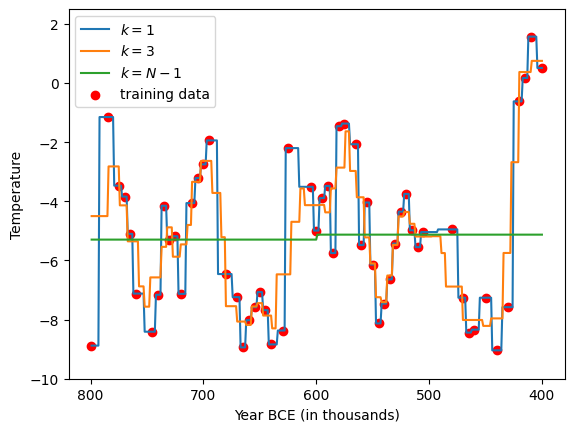
\includegraphics[width=0.5\linewidth]{img_output/p1.1a.png}
            \caption{k-Nearest Neighbors}
            \label{fig:enter-label}
        \end{figure}

        \item 
        MSE for k = 1: 1.74
        \\MSE for k = 3: 3.89
        \\MSE for k = N-1: 9.73
        \\ The solution with the lowest MSE is $k=1$. Thus clearly the test data has comparable trends to the training data, and our worry about this model potentially overfitting are somewhat assuaged. 
        
    \end{enumerate}

    \item 
    \begin{enumerate}
        \item As $\tau$ increases, the model decays at a slower rate. This means that for the low values of $\tau$ like $\tau = 1$, the kernel function decays fast and thus puts more emphasis on points closer to the input value. This is why on the graph you can see a more jagged plot, and one that fits closer to the individual data points around it. For $\tau =50$ the fit is a little smoother. This will decay a little slower, which means that the proportion of the weights placed on points close to the input value versus those further away is closer to 1, and thus will smooth out the plot more. With the largest $\tau$, $\tau = 2500$, it still puts more weight on those closer to the input value than those further away, however, it incorporates the values further away more than the other $\tau$ values. This results in a less dramatic plot as the changes in the input value have less difference in the weights of which points are emphasized because they are all more equally recognized. 
        \begin{figure}[htp]
            \centering
            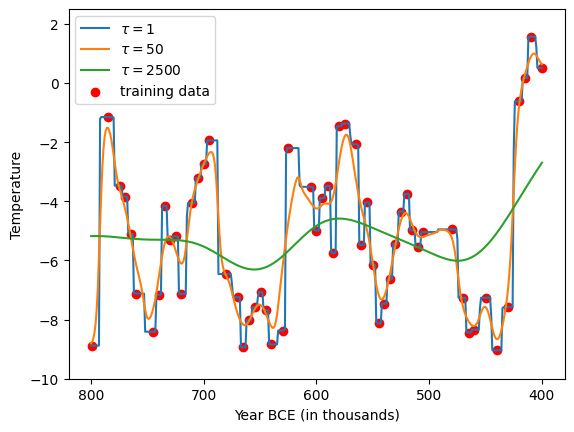
\includegraphics[width=0.5\linewidth]{img_output/p1.2a.png}
            \caption{Kernelized Regression}
            \label{fig:enter-label}
        \end{figure}
        \\\\\\\\
        \item
        $$\text{MSE} = \frac{1}{M}*\sum_{m=1}^M(\frac{\sum_{n=1}^N K_{\tau}(x_n, x_m')y_n}{\sum_{n=1}^N K_{\tau}(x_n, x_m')} - y_m')^2 $$
        
        \item 
        MSE for $\tau = 1: 1.95$
        \\MSE for $\tau = 50: 1.86$
        \\MSE for $\tau = 2500: 8.33$
        \\ The model with the lowest MSE is when $\tau = 50$. This makes sense, because it is the model that is capable of recognizing the variance in the dataset, without being too locked into the given data points as to be overfit. We can see that it captures the trends of the data well, without being overly complex, which demonstrates it will generalize well (as we see by it having the lowest MSE). We do not want to choose our $\tau$ value based on $\mathcal{D}_\texttt{train}$ because that is what our model is trained on, thus if we were to see which model (i.e. which $\tau$) fits that data the best, it will obviously be the one fits exactly to the given data (i.e. $\tau = 1$). However, we want a model that has predictive power beyond the given data, and so fitting the training data exactly, is not a good thing in most cases. As such, we should choose $\tau$ based on its predictive capabilities outside our training data, using a test set. 

        \item
        The time and space complexities of kernelized regression grow linearly. Finding all of the kernel weights, relies on calculations with all of the training points, thus is $O(N)$, in both time and space, as you need $O(N)$ calculations (time) and need to store those weights, and the actually training data  (space). Then when actually calculating the prediction $f_{\tau}(x^*)$ for $x^*$, you rely on all of those weights (i.e. $O(N)$ again). In the end, growth in the size of training set, increases the time and space complexity linearly as it relies on all of the training points for calculations. 
        \\ For kNN, the growth of complexities is also linear to some extent (depends a little on implementation). You have to check the distances to every point in training set ($O(N)$), in order to find the k-nearest neighbors. There is some pre-processing that you could do to reduce the complexity of this by ordering your training points, and doing a reduction to sorting for finding the nearest neighbors, however using the implementation provided, calculations with all training points is necessary. Furthermore, the sorting of distances after each calculation is $O(n\log n)$, so does not affect the asymptotic complexity. Then the final prediction calculation is more dependent on $k$ ($T_{f_{\tau}} = O(k)$). Which, if $k=N$ then you will rely on all of the training points. Meaning a larger $N$ means more time and space complexity (also linear in growth).

        \item As $\tau \rightarrow 0$ then the kernel function will go to 0 at a really fast pace when the value of $(x-x')^2$ increases. This results in a highly peaked function that decays really fast. This means that the Kernel function will assign tangible weights to the nearest points, and near 0 weights to anything remotely distanced. The largest weight $K(x,x^*)= \exp (-\frac{(x-x^*)^2}{\tau})$ will occur when $\frac{(x-x^*)^2}{\tau}$ is the smallest value. Since $\tau \rightarrow 0$ then we need the denominator to be really small in order to offset dividing by a small number. This will only occur when $(x-x^*)$ is a small number (i.e. $x$ and $x^*$ are very close to each other). This results in $f_{\tau}(x^*) = y_{n^*}$ where $y_{n^*}$ is the output value of the point closest to $x^*$. Any point that is not the nearest point will have a proportionally tiny weight comparatively thus will have little to no effect.
        
    \end{enumerate}
\end{enumerate}

\end{solution}


%%%%%%%%%%%%%%%%%%%%%%%%%%%%%%%%%%%%%%%%%%%%%
% Problem 2
%%%%%%%%%%%%%%%%%%%%%%%%%%%%%%%%%%%%%%%%%%%%%
\newpage
\begin{problem}[Deriving Linear Regression, 20pts]

We now seek to model the temperatures with a parametric method: linear regression. Before we implement anything, let's revisit the mathematical formulation of linear regression.  Specifically, the solution for the least squares linear regression  ``looks'' kind of like a ratio of covariance and
variance terms.  In this problem, we will make that connection more
explicit. \\

\noindent Suppose we have some 2-D data where each observation has the form $(x, y)$ and is independent and identically distributed according  $x \sim p(x)$, $y \sim p(y|x)$. We will consider the process of fitting these data from this distribution with the best linear model
possible, that is a linear model of the form $\hat{y} = wx$ that
minimizes the expected squared loss $E_{x,y}[ ( y - \hat{y} )^2
    ]$.\\

\noindent Note: The notation $E_{x, y}$ indicates an
expectation taken over the joint distribution $p(x,y)$. This essentially just means to treat $x$ and $y$ as random.  

\begin{enumerate}

  \item Derive an expression for the optimal $w$, that is, the $w$
        that minimizes the expected squared loss above.  You should leave
        your answer in terms of moments of the distribution, e.g. terms
        like $E_x[x]$, $E_x[x^2]$, $E_y[y]$, $E_y[y^2]$, $E_{x,y}[xy]$
        etc.

  \item Note that while $x, y$ are data that we have access to, $E_{x, y}[yx]$ is a theoretical constant. Keeping in mind the interpretation of expectations as average values, how could you use observed data $\{(x_n,y_n)\}_{n=1}^N$ to estimate $E_{x, y}[yx]$ and $E_x[x^2]$?

  \item In general, moment terms like $E_{x, y}[yx]$, $E_{x, y}[x^2]$,
        $E_{x, y}[yx^3]$, $E_{x, y}[\frac{x}{y}]$, etc. can easily be
        estimated from the data (like you did above).  If you substitute in
        these empirical moments, how does your expression for the optimal
        $w^*$ in this problem compare with the optimal $\bm{\hat w}$ from Problem 4.3 of HW0?

  \item Many common probabilistic linear regression models assume that
        variables $x$ and $y$ are jointly Gaussian.  Did any of your above
        derivations rely on the assumption that $x$ and $y$ are jointly
        Gaussian?  Why or why not?
\end{enumerate}
\end{problem}

\newpage
\begin{solution}
	\begin{enumerate}
	    \item To derive the optimal $w$ that minimizes the expected        squared loss lets first put $\hat{y}$ and $y$ in terms of          moments of the distribution. 
            $$E_{x,y}[(y-\hat{y})^2]=E[(y-wx)^2]=E[y^2-2wxy+w^2x^2]$$
            Linearity of expectation can separate the arithmetic
            $$E[y^2-2wxy+w^2x^2]= E[y^2]-2wE[xy]+w^2E[x^2]$$
            To find optimal $w$ set the derivative with respect to $w$ equal to 0.
            $$\frac{d(E[y^2]-2wE[xy]+w^2E[x^2])}{dw} = 0 = -2E_{x,y}[xy]+2wE_x[x^2]$$
            $$w = \frac{E_{x,y}[xy]}{E_x[x^2]}$$

            \item In order to estimate $E_x[x^2]$ and $E_{x,y}[xy]$ based on the observed data, you can use sums to find the averages in the data. 
            $$E_x[x^2] = \frac{1}{N}\sum_{n=1}^N x_n^2$$
            $$E_{x,y}[xy] = \frac{1}{N}\sum_{n=1}^N x_ny_n$$

            \item Substituted in $$w^* = \frac{\frac{1}{N}\sum_{n=1}^N x_ny_n}{\frac{1}{N}\sum_{n=1}^N x_n^2}$$
            $\hat{w}$ in HW0 was $\bm{\hat w} = (\bm X^\top \bm X)^{-1}\bm X^\top \bm y$, which if we were to use just a singular moment, that is, a singular column vector for $x$ then $\bm X^\top \bm X = \sum_{n=1}^N x_n^2$, and the inverse is $\frac{1}{\sum_{n=1}^N x_n^2}$. Second $\bm X^\top \bm y = \sum_{n=1}^N x_ny_n$ and put together: 
            $$\frac{1}{\sum_{n=1}^N x_n^2} * \sum_{n=1}^N x_ny_n$$
            Which is equivalent to our optimal $w^*$ above.

            \item No none of the above derivations relied on assumptions that $x$ and $y$ are jointly Gaussian. This is because our moment terms, which are just expectations, are simply sums that are used similarly with all distributions. The rest of the derivations simply relied on laws of Expectations which do not change.  
	\end{enumerate}
\end{solution}

%%%%%%%%%%%%%%%%%%%%%%%%%%%%%%%%%%%%%%%%%%%%%
% Problem 3
%%%%%%%%%%%%%%%%%%%%%%%%%%%%%%%%%%%%%%%%%%%%%

\begin{problem}[Basis Regression, 30pts]

 Having reviewed the theory, we now implement some linear regression models for the temperature. If we just directly use the data as given to us, we would only have
    a one dimensional input to our model, the year.  To create a more expressive linear
    model, we will introduce basis functions.

\vspace{1em}

\noindent\emph{Make sure to include all required plots in your PDF.}

\begin{enumerate}
  \item
        We will first implement the four basis regressions below. (The first basis has been implemented for you in the notebook as an example.) Note that we introduce an addition transform $f$ (already into the provided notebook) to address concerns about numerical instabilities.
        \begin{enumerate}
          \item $\phi_j(x)= f(x)^j$ for $j=1,\ldots, 9$. $f(x) = \frac{x}{1.81 \cdot 10^{2}}.$
          \item $\phi_j(x) = \exp\left\{-\cfrac{(f(x)-\mu_j)^2}{5}\right\}$ for $\mu_j=\frac{j + 7}{8}$ with $j=1,\ldots, 9$. $f(x) = \frac{x}{4.00 \cdot 10^{2}}.$
          \item $\phi_j(x) =  \cos(f(x) / j)$ for $j=1, \ldots, 9$. $f(x) = \frac{x}{1.81}$.
          \item $\phi_j(x) = \cos(f(x) / j)$ for $j=1, \ldots, 49$. $f(x) = \frac{x}{1.81 \cdot 10^{-1}}$. \footnote{For the trigonometric bases (c) and (d), the periodic nature of
                  cosine requires us to transform the data such that the
                  lengthscale is within the periods of each element of our basis.}
        \end{enumerate}

        {\footnotesize * Note: Please make sure to add a bias term for
        all your basis functions above in your implementation of the
        \verb|make_basis|.}

        Let
        $$ \mathbf{\phi}(\mathbf{X}) =
          \begin{bmatrix}
            \mathbf{\phi}(x_1) \\
            \mathbf{\phi}(x_2) \\
            \vdots             \\
            \mathbf{\phi}(x_N) \\
          \end{bmatrix} \in \mathbb{R}^{N\times D}.$$
        You will complete the \verb|make_basis| function which must return
        $\phi(\mathbf{X})$ for each part
        (a) - (d). You do NOT need to submit this
        code in your \LaTeX writeup.

        Then, create a plot of the fitted
        regression line for each basis against a scatter plot
        of the training data. Boilerplate plotting code is provided in the
        notebook---you will only need to finish up a part of it.
        \textbf{All you need to include
          in your writeup for this part are these four plots.}

        \item
          Now we have trained each of our basis regressions. For each basis
          regression, compute the MSE on the test set.  Discuss: do any of the
          bases seem to overfit?  Underfit?  Why?


    \item Briefly describe what purpose the transforms $f$ serve: why are they helpful?

    \item As in Problem 1, describe the space and time complexity of linear regression.  How does what is stored to compute predictions change with the size of the training set $N$ and the number of features $D$?  How does the computation needed to compute the prediction for a new input depend on the size of the training set $N$?  How do these complexities compare to those of the kNN and kernelized regressor?

    \item Briefly compare and constrast the different regressors: kNN,
          kernelized regression, and linear regression (with bases).  Are some
          regressions clearly worse than others?  Is there one best
          regression?  How would you use the fact that you have these multiple
          regression functions?

  \end{enumerate}
  Note:
  Recall that we are using a
  different set of inputs $\mathbf{X}$ for each basis (a)-(d).
  Although it may seem as though this prevents us from being able
  to directly compare the MSE since we are using different data,
  each transformation can be considered as being a part of our model.
  Contrast this with transformations (such as standardization) that cause the variance of the target $\mathbf{y}$ to be different; in these cases the
  MSE can no longer be directly compared.
\end{problem}

\newpage 
\begin{solution}
	\begin{enumerate}
	    \item These are the resulting plots  
                \begin{figure} [htp] \centering                             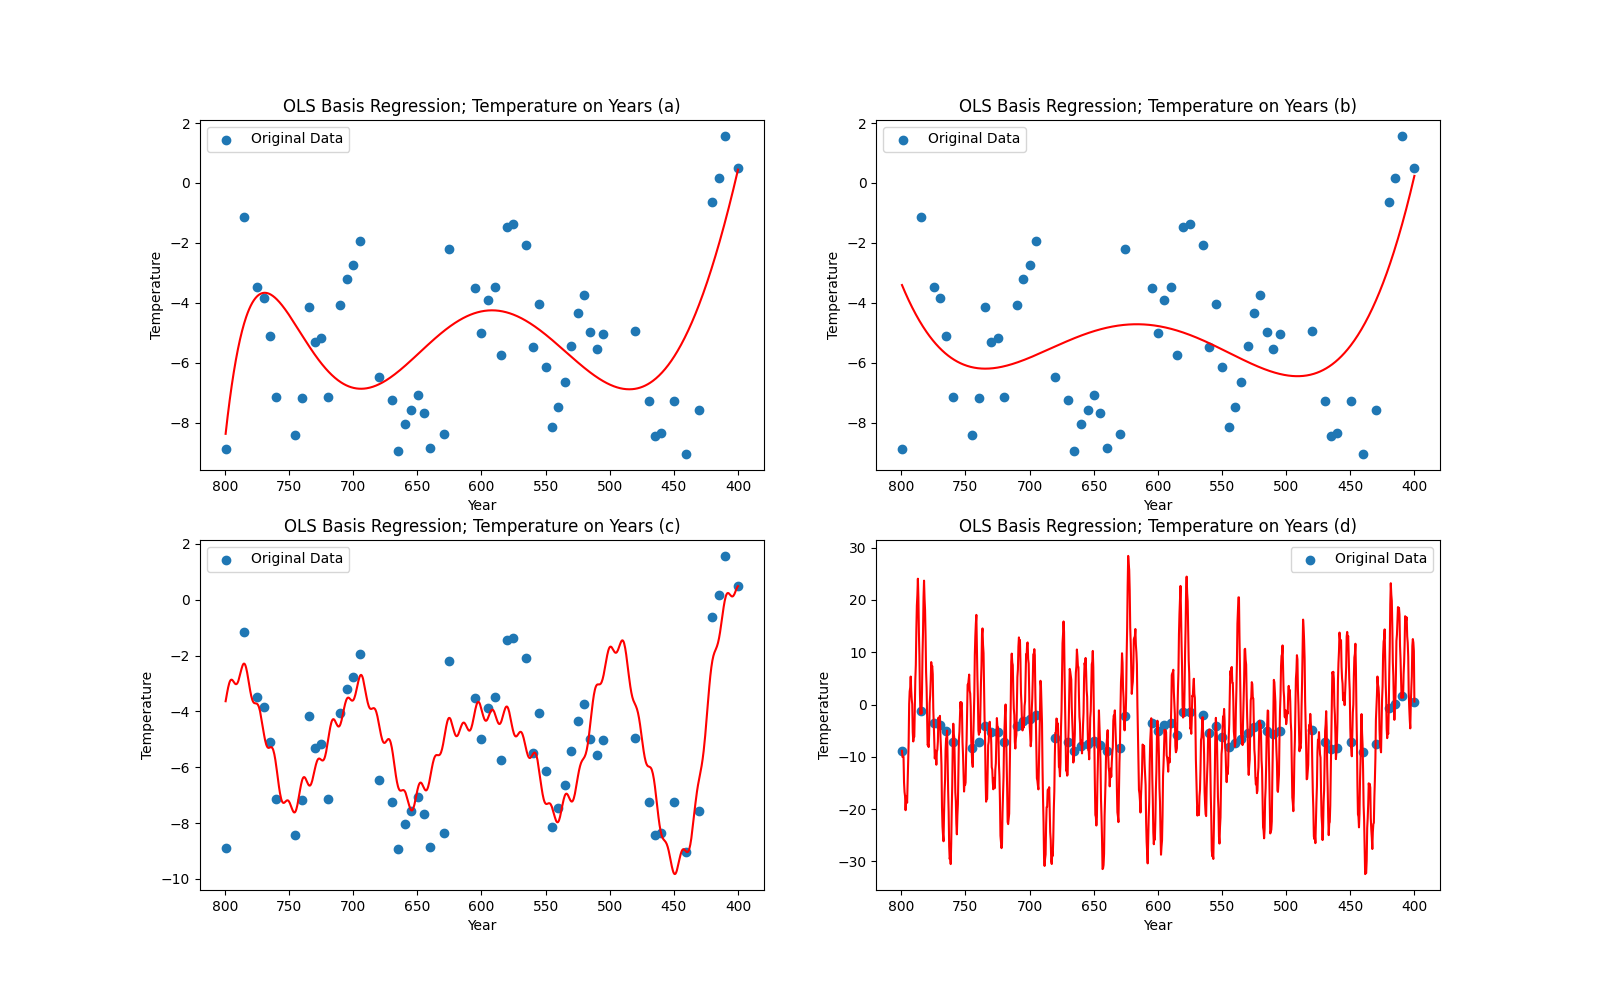
\includegraphics[width=0.8\linewidth]{img_output/p3.1.png} \caption{Basis Regression Plots} \label{fig:enter-label} \end{figure}

            \item Here are the resulting test-set MSE values:
            \\ MSE for part a: 7.96
            \\ MSE for part b: 8.71
            \\ MSE for part c: 5.97
            \\ MSE for part d: 58.89
            \\ I suspect that part d is overfit. Part d, has a very high test MSE value, and after calculating its training MSE (0.64), it is quite clearly overfit. Looking at the plot we can see that it is extremely complex in order for the model to accurately incorporate every data point in the training data. However, this jeopardizes its generalizability in the test set. I suspect that part b, and even maybe part a, could be argued as underfit, as their MSEs are not as low as part c. Furthermore, their plots look unconvincing in their ability to capture any trends (especially true for part b). That being said, just looking at the original data, there are not the most clear trends in the data. Part c however, has the best test data MSE and seems to have some level of complexity without being too biased to noise in the training data (Goldilocks zone). 

            \item The transformations $f$ serve to incorporate more information into the training set. They map the data into  higher dimension where a linear regression model may be suitable. In many cases, the data, in its original form, does not show linear trends (as we can see with this problem), however, choosing ways to map it into higher dimensions (our different basis functions), can map the data into a dimension that it may be more linear. It does not change the underlying shape of the data, but simply allows the model to be more complex via increased dimensionality (while still staying linear in those higher dimensions). As such we can still use a linear model, but perform an effective regression on more complex data trends. 

            \item The space complexity of linear regression is simply storing the training set (N). Since this is what the model is trained on it needs to store those values, however once finished training it is no longer necessary and only the weights must be stored, which will be of size D. This is because if each data point has D features, then there has to be an associated D features/weights in $\textbf{w}$. As $N$ increases, the space complexity for training increases linearly with $O(N)$ growth as well as $O(D)$ depending on whether $D$ is also increasing. However, only a vector of size $D$ is necessary to be stored for predictions. Then for time complexity, we use the closed solution of $\bm{\hat w} = (\bm X^\top \bm X)^{-1}\bm X^\top \bm y$. The inversion of a matrix is a long series of arithmetic and is $D^3$ time complexity. Then the heavy matrix multiplication of $N\text{x}D$ matrices takes $O(ND^2)$. The dominant time complexity is then one which is bigger $D^3$ or $ND^2$. Then in order to execute predictions you simply have $D$ operations for each of the features in an input value, and is not dependent on the size of training set other than the number of features each training point has.
            \\\\
            Whereas kNN and kernelized regression require all the training data points for every prediction calculation, linear regression does not. This means the space complexity is greater for those methods after training. With that being said, linear regression requires more extensive training calculation (time complexity), as described above, assuming for kNN and kernelized regression you have $k$ and $\tau$ set. In terms of time complexity for prediction, it is a similar story. Linear regression is $O(D)$ calculations for predictions, kernelized regression is $O(ND)$ (computing the kernel is this complexity), and kNN is $O(ND + N\log N)$ (finding distances, and sorting). 

            \item When looking to compare these methods you are balancing 3 factors. 1) Actual predictive performance 2) Time and space complexity 3) Frequency of predictions. Obviously the priority is predictive performance, but maybe you would be willing to sacrifice a little bit of performance in return lower time and space complexity. Furthermore, when comparing models, with similar predictive capability, an important thing to recognize is will you be predicting often or just once. If it is often then, linear regression is likely a better choice, because it has a heavier pre-processing complexity, but once the weights are established the prediction calculations are much less, so over time you save complexity over the other methods. On the other hand, if you only need to predict once, then maybe kernelized regression or kNN is better to avoid heavier pre-processing costs in linear regression (holding predictive performance constant). I would argue that there is no one model that is better or worse, it simply relies on the priorities that an investigator is recognizing as they are building the model. Thus since you have these multiple regression functions, you should be able to recognize which method works best for your situation. 
            
        \end{enumerate}
\end{solution}

%%%%%%%%%%%%%%%%%%%%%%%%%%%%%%%%%%%%%%%%%%%%%
% Problem 4
%%%%%%%%%%%%%%%%%%%%%%%%%%%%%%%%%%%%%%%%%%%%%
\begin{problem}[Probablistic Regression and Regularization, 30pts]

Finally, we will preview Bayesian regression and explore its connection to regularization for linear models. Then, we will fit a regularized model to the temperature data. Although the content is related, you do not need to know the material from the lectures on frequentist model selection and Bayesian model selection to solve this problem.  \\

\noindent Recall that the probabilistic version of linear regression states that 
\[y_n = \boldw^\top\boldx_n + \epsilon_n, \quad \epsilon_n \sim \mathcal{N}(0, \sigma^2)\]
In Bayesian regression, we impose a prior $p(\boldw)$ on the weights and  fit the weights $\boldw$ through maximizing the posterior likelihood
\[p(\boldw | \boldX, \boldy) = \frac{p(\bold y | \boldw, \boldX)p(\boldw)}{p(\boldy | \boldX)}\]
Note: since we maximize with respect to $\boldw$, it suffices to just maximize the numerator.

\begin{enumerate}
    \item Suppose $\boldw \sim \mathcal{N}(\mathbf{0},\frac{\sigma^2}{\lambda}\boldI)$. Show that maximizing the posterior likelihood is equivalent to minimizing 
    \[\mathcal{L}_{ridge}(\boldw) = \frac{1}{2}||\boldy -\bold X\boldw||_2^2 + \frac{\lambda}{2}||\boldw||_2^2.\] 
    Note that minimizing $\mathcal{L}_{ridge}(\boldw)$ is exactly what ridge regression does.
    
    Hint: You don't need to solve for the maximizer/minimizer to show that the optimization problems are equivalent.
    
    \item Solve for the value of $\boldw$ that minimizes $\mathcal L_{ridge}(\boldw)$.

    \item The Laplace distribution has the PDF
   \[L(a,b) =\frac{1}{2b} \exp\left(-\frac{|x - a|}{b}\right)\]
Show that if all $w_d \sim L\left(0,\frac{2\sigma^2}{\lambda}\right)$, maximizing the posterior likelihood is equivalent to minimizing 
\[\mathcal{L}_{lasso}(\boldw) = \frac{1}{2}||\boldy -\bold X\boldw||_2^2  + \frac{\lambda}{2}||\boldw||_1.\] 
Note that minimizing $\mathcal{L}_{lasso}(\boldw)$ is exactly what LASSO regression does.

    \item Why is there no general closed form for the LASSO estimator, i.e. the value of $\boldw$ that minimizes $\mathcal{L}_{ridge}(\boldw)$?

    \item Since there is no general closed form for LASSO, we use numerical methods for estimating $\boldw$. One approach is to use \textit{coordinate descent}, which works as follows: 
    \begin{enumerate}
        \item Initialize $\boldw=\boldw_0$.
        \item For each $d=1, \ldots, D$ do the following 2 steps consecutively:
        \begin{enumerate}
            \item Compute $\rho_d = \tilde{\boldx}_d^\top(\boldy - (\boldX \boldw - w_d \tilde{\boldx}_d))$. We define $\tilde{\boldx}_d$ as the $d$-th column of $\boldX$.

            \item If $d=1$, set $w_1 = \frac{\rho_1}{||\tilde{\boldx}_1||^2_2}$. Otherwise if $d\ne 1$, compute $w_d = \frac{\text{sign}(\rho_d)\max\left\{|\rho_d|-\frac{\lambda}{2}, 0\right\}}{||\tilde{\boldx}_d||^2_2}$.
        \end{enumerate}
        \item Repeat step (b) until convergence or the maximum number of iterations is reached.
    \end{enumerate} 

    Implement the \texttt{find\_lasso\_weights} function according to the above algorithm, letting the max number of iterations be 5000. Then, fit models with $\lambda=1, 10$ to basis (d) from Problem 3, plot the predictions, and compute the MSE's. You will need to do some preprocessing, but a completed helper function for this is already provided. How do the graphs and errors compare to those for the unregularized basis (d) model? 


\end{enumerate}

\end{problem}

\newpage
\begin{solution}
	\begin{enumerate}
	    \item Since we only need to maximize with respect to $\textbf{w}$ then we focus on the numerator of the posterior distribution. $$p(\textbf{y}|\textbf{w},\textbf{X})p(\textbf{w}) = $$ 
        
        $$p(\textbf{y}|\textbf{X},\textbf{w}) = \mathcal{N}(\textbf{y}|\textbf{Xw}, \sigma^2\textbf{I})$$
        $$p(\textbf{w}) = \mathcal{N}(\textbf{w}|0, \frac{\sigma^2}{\lambda})$$
        Then on the likelihood side: $$p(\textbf{y}|\textbf{w},\textbf{X}) = \frac{1}{(2\pi\sigma^2)^{N/2}}\exp(\frac{-1}{2\sigma^2}||\textbf{y} - \textbf{Xw}||_2^2$$
        N is the number of data points. 
        $$p(\textbf{w}) = \frac{1}{(2\pi\sigma^2/\lambda)^{D/2}}\exp(\frac{-\lambda}{2\sigma^2})||\textbf{w}||_2^2$$
        D is dimensionality of the weight vector $\textbf{w}$. Now we will take the log of the complete posterior term (importantly we are also dropping constants that do not depend on y in the first term and w in the second):
        $$\log(p(w|X,y))\propto\log(p(y|X,w)p(w)= -\frac{1}{2\sigma^2}||\textbf{y} - \textbf{Xw}||^2_2-\frac{\lambda}{2\sigma^2}||\textbf{w}||^2_2 + constant$$
        Finally we take the negative of the function. This is where we switch from maximizing to minimizing as taking the negative of a function switches the direction of optimization (i.e. maximizing to minimizing).
        $$\log(p(y|X,w)p(w)= \frac{1}{2\sigma^2}||\textbf{y} + \textbf{Xw}||^2_2-\frac{\lambda}{2\sigma^2}||\textbf{w}||^2_2 + constant$$
       This is equivalent to the $\mathcal{L}_{ridge}(\boldw)$ term. We can see that there are additional $\sigma^2$, but when optimizing these are canceled as they are constant factors not dependent on $w$. Futhermore, we are minimizing this function, because when we take the negative log, we flip the optimization problem from maximizing the posterior, to minimizing the negative log-posterior

        \item To solve for value of $\textbf{w}$ that minimizes $\mathcal{L}_{ridge}(\boldw)$, we set its derivative equal to 0. 
            $$\frac{d\mathcal{L}}{dw} = 0 = d/dw(\frac{1}{2}(\textbf{y} -\textbf{Xw})^\top(\textbf{y} -\textbf{Xw})+\frac{\lambda}{2} \textbf{w}^\top\textbf{w})$$
            $$d/dw(\frac{1}{2}(\textbf{y}^\top\textbf{y}-2\textbf{y}^\top\textbf{Xw}) + \textbf{Xw}^\top\textbf{Xw} +\frac{\lambda}{2} \textbf{w}^\top\textbf{w}) = -\textbf{y}^\top\textbf{X}+\textbf{X}^\top\textbf{Xw}+\lambda\textbf{w} = 0$$
            simplifying...
            $$\textbf{X}^\top\textbf{Xw}+\lambda\textbf{w} = \textbf{yX}^\top$$
            solve for $\textbf{w}$...
            $$\textbf{w}(\textbf{X}^\top\textbf{X}+\lambda\textbf{I})=\textbf{X}^\top\textbf{y}$$
            $$\textbf{w} = (\textbf{X}^\top\textbf{X}+\lambda\textbf{I})^{-1}\textbf{X}^\top\textbf{y}$$

            \item 
            The first term ($p(\textbf{y}|\textbf{X}, \textbf{w})$) of the posterior distribution ($p(\textbf{w}|\textbf{y}, \textbf{X}$)) remains the same because even though here we are using a different distribution of $\textbf{w}$ that first term is conditioned on $\textbf{w}$. Thus we will focuse on the second term of the posterior distribution ($p(\textbf{w})$). The PDF of the Laplace distribution for $w_d$ is $=\frac{1}{2b}\exp(-\frac{|x-a|}{b})$
            thus $\textbf{w}$ with $w_d \sim L\left(0,\frac{2\sigma^2}{\lambda}\right)$ is
            $$p(\textbf{w}) = \prod_{d=1}^D\frac{\lambda}{2\sigma^2}\exp(-\frac{\lambda}{2\sigma^2}|w_d|)$$
            We can take the log to get rid of the products and reduce the exponential. 
            $$\log p(\textbf{w}) = - \frac{\lambda}{2\sigma^2}||\textbf{w}||_1$$
            Lets combine it back with the first term (we will have taken the log already to that term). Thus
            $$\log p(\textbf{w}|\textbf{X},\textbf{y}) = -\frac{1}{2\sigma^2}||\textbf{y}-\textbf{Xw}||^2_2-\frac{\lambda}{2\sigma^2}||\textbf{w}||_1$$
            Similar to above, we now take the negative to switch the direction of optimization. So instead of maximizing we are now minimizing. 
            $$\log p(\textbf{w}|\textbf{X},\textbf{y}) = \frac{1}{2\sigma^2}||\textbf{y}-\textbf{Xw}||^2_2+\frac{\lambda}{2\sigma^2}||\textbf{w}||_1$$
            This is the same as minimizing $\mathcal{L}_{lasso}(\boldw)$. Also similar to above, we are left with $\sigma^2$ terms, but when we are optimizing, these constant factors, and thus will cancel out when solving for an optimal w.
            \item The reason there is no general closed form for the LASSO estimator is because when we introduce that the PDF of $w$ as the Laplace distribution $\prod_{d=1}^D\frac{\lambda}{2\sigma^2}\exp(-\frac{\lambda}{2\sigma^2}|w_d|)$, which introduces a L1 term, that is, an absolute value term. This means that the function is no longer differentiable at 0, and as a result we cannot find a gradient with respect to w. As such there will not be a closed form solution, only iterative methods to narrow in on the optimal weights. 

            \item Here are the plots of the fitted models. 
            \begin{figure}[htp]
                \centering
                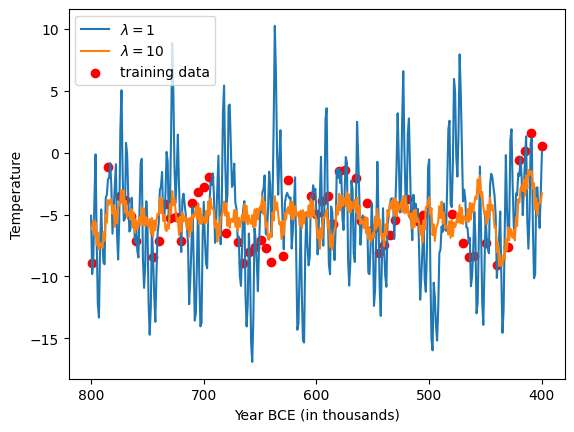
\includegraphics[width=0.5\linewidth]{img_output/p4.5.png}
                \caption{Lasso Regression}
                \label{fig:enter-label}
            \end{figure}

            The resulting test MSE values were:
            \\ $\lambda = 1$ : $19.27$
            \\ $\lambda = 10$: $10.03$
            \\ This shows that the reduced dimensionality/complexity due to LASSO regression, helped improve the MSE significantly. Before, the MSE was $58$, and now with $\lambda=10$ it was reduced to $10.03$, a major improvement. With that being said, looking at the plot, I do not think it captures the trends that well, and may simply have improved accuracy by having less variance and staying more centralized to the plot. Nonetheless, this method did help in the end, and it does capture the trends in some regard. 

            
	\end{enumerate}
\end{solution}


%%%%%%%%%%%%%%%%%%%%%%%%%%%%%%%%%%%%%%%%%%%%%
% Name and Calibration
%%%%%%%%%%%%%%%%%%%%%%%%%%%%%%%%%%%%%%%%%%%%%
\newpage
\subsection*{Name} Ethan Veghte

\subsection*{Collaborators and Resources}
Whom did you work with, and did you use any resources beyond cs181-textbook and your notes?


\end{document}
